\hypertarget{nbirdt}{%
\chapter{New Brunswick Institute for Research, Data and Training: A Ten-Year Partnership Between Government and Academia}\label{nbirdt}}

\printchapterauthor{%
\begin{authorlist}
  Donna Curtis Maillet (University of New Brunswick)  \\
  James Ted McDonald (University of New Brunswick)  \\
\end{authorlist}}\authorfootnote{Curtis Maillet, Donna,  and James Ted McDonald}{Donna Curtis Maillet and James Ted McDonald}{nbirdt}
\authortoc{Donna Curtis Maillet, James Ted McDonald}
\hrulefill

\hypertarget{nbirdt-summ}{%
\section{Summary}\label{nbirdt-summ}}

This case study describes the establishment and development of the New Brunswick Institute for Research, Data and Training (NB-IRDT) in Fredericton, NB, Canada. NB-IRDT is a provincial research data center and data custodian as defined in NB legislation and is the product of an extensive and ongoing collaboration between the Government of New Brunswick (GNB) and academic members of the University of New Brunswick (UNB) among others. Launched in 2015 with the delivery of the first data set, NB-IRDT now holds and provides research access to more than 45 linkable person-level data sets from across the spectrum of service provision in NB. This includes access to data on health, social assistance, education and training, aged care, and workers compensation. Data sets are provided from government agencies and other public bodies as well as non-profit organizations. The case study highlights notable or unique aspects of NB-IRDT and describes the context of how those aspects came to be part of NB-IRDT policy. Aspects of particular note are (1) the legal authority NB-IRDT has to receive, hold, and provide access to personal level linkable data from across NB public bodies, (2) data access that is not restricted to academic users but also users from government, the non-profit sector, and the private sector without a required affiliation to UNB, and (3) active engagement with senior government decision-makers in collaborative research programs focused on government priority areas.

\hypertarget{nbirdt-intro}{%
\section{Introduction}\label{nbirdt-intro}}

\hypertarget{nbirdt-motivation}{%
\subsection{Motivation and Background}\label{nbirdt-motivation}}

The impetus for the collaboration that would lead to the establishment of NB-IRDT was a recognition by certain key senior provincial civil servants following the financial crisis of 2007 to 2008 that evidence to support much government expenditure to deliver healthcare, education and training, and social programs\footnote{In Canada, provincial governments have responsibility for providing services in these three key areas and as a result, spending on health, education, and income support consumes much of a province's budget. For 2019, two-thirds of the NB budget was forecast to be spent in these areas.} was lacking. Although large amounts of data were being collected by government agencies, institutional barriers such as separate IT systems, and legal barriers such as restrictions on inter-institutional data sharing, meant that personal data could not easily be shared between those agencies. At the same time, successive years of civil service cutbacks had markedly reduced government's capacity to undertake research and program evaluation itself. In the words of one deputy minister, ``We have spent CA\$2 billion over the last ten years on programs and still have no idea what has worked.''\footnote{Personal correspondence between Ted McDonald and Jean-Marc Dupuis, March 2018.} Compounding the need for action were mounting fiscal and demographic pressures on the provincial budget: NB is small (population in 2019 was less than 750,000), is almost 50 percent rural, has one of the most rapidly aging population profiles in Canada, and has relatively high rates of obesity and chronic disease such as diabetes and chronic obstructive pulmonary disease \citep{statisticscanada2020}. At the same time, researchers seeking to undertake work using provincial administrative data were required to follow a time-consuming and opaque process that put significant resource demands both on the applicant and on the department from which data were sought. Opportunities to access linked data from multiple departments and public bodies were negligible. Similarly, internal government staff faced similar difficulties with gaining access to data from multiple agencies, meaning that most of the research that did occur was siloed within particular agencies.

Although it would be five years between initial conception of the idea for NB-IRDT and receipt of the first administrative data set in 2015, certain core principles guided development. The first of these was that any research undertaken should be credible, independent, transparent, and rigorous. This would lead to more informed decision-making where the public and other stakeholders would have confidence that sound and unbiased research had been provided to those decision-makers. The institute would thus be situated in a university where the institute leadership answered to the vice president (research) and not government. It would also be empowered to act as data custodian and have the right to grant and control access to administrative data for legitimate research purposes. Furthermore, while government would have an active role in the setting of research priorities and in the review of particular proposals, it would not have veto power, nor could it veto the dissemination of research results. Instead, a rigorous approval process was jointly developed that respected privacy, ensured only legitimate research (where research is broadly defined) was conducted, and that academic freedom was enshrined. As NB-IRDT developed, these policies continued to evolve to reflect the five safes framework to be discussed in more detail below.

The second principle was that NB-IRDT would be a resource for the Province of NB and would not be only a UNB facility. With four major universities, two medical schools, and two regional health authorities all research active in the health domain, this data resource would need to be available to all. Although it would be established within UNB, right of access to data for research was not restricted to UNB researchers nor even academic researchers. As long as the proposed research had legitimate research inquiry goals, there were no restrictions on who could request access to the data: individuals from academic, public, private, and non-profit sectors from NB and elsewhere could all do so as long as they followed the prescribed data access protocol. At the same time, NB-IRDT was left to develop its own fee structure to support the longer-term sustainability of the Institute.

The third principle was that for government to reap the full benefits of providing data to support policymaking, data needed to be linkable at the individual level and span the range of government service provision. Thus, the Province of NB undertook to support data transfer to NB-IRDT where the onus would be on individual agencies to demonstrate why particular data elements would not be transferred rather than on NB-IRDT to justify why they should. In other words, the government committed to the eventual transfer of all research-relevant data, and this was extended to include all public bodies in NB. NB-IRDT would in turn assume the responsibility of ensuring minimum required data disclosure to researchers for approved projects. Parallel to this, although NB lacked a universal personal identifying number for all government services, there was agreement that the provincial health insurance (Medicare) number would provide the index backbone to allow all data to be made linkable at the individual level. The Department of Health undertook to provide this corporate function for NB-IRDT and public bodies seeking to disclose data so that although researchers could access linked data files, neither NB-IRDT nor researchers accessing data through it would see Medicare numbers.

A fourth principle was that no government department or public body would be compelled to enter into data sharing agreements with NB-IRDT, though if they did it was understood that they would transfer close to complete data sets to the NB-IRDT platform. In every case, the decision to transfer data to NB-IRDT would remain the decision of the agency's senior decision-maker (deputy ministers in the case of GNB departments). It would fall to NB-IRDT, its Government champions, and the wider research community to make the case that doing so would be in the interest of the disclosing entity.

\hypertarget{nbirdt-examples}{%
\subsection{Data Use Examples}\label{nbirdt-examples}}

NB-IRDT represents a transformation in health and social science research infrastructure in NB and as of June 2020 holds more than forty administrative data sets spanning hospitalizations, immigrant arrivals, cancer screening, post-secondary training, long term care facilities, K--12 school report cards, and many other topics. In addition, more than fifty research projects have been initiated, are in progress, or have been completed since 2015, involving academic, clinical health, government, and private sector researchers.\footnote{See NB-IRDT \href{https://www.unb.ca/nbirdt/}{website} for more details.} Much of the research in the health domain has been undertaken under the auspices of a research collaboration with the Department of Health through the \href{https://cihr-irsc.gc.ca/e/45859.html}{Canadian Institutes of Health Research (CIHR)} \href{http://www.spor-maritime-srap.ca/}{Strategy for Patient-Oriented Research (SPOR)}. The SPOR\index{SPOR} Support Unit program, of which the Maritime SPOR SUPPORT Unit\index{Maritime SPOR SUPPORT Unit} (MSSU) is a key element, involves equal contributions of federal and provincial funding and is described in detail elsewhere. Projects underway or completed include examinations of the impact of surgical experience on patient outcomes, the effects on health service use of rural hospital closure, and a series of projects on the effects of air quality, living in proximity to green space and blue space, and industrial emissions on different dimensions of health and mortality. Another project underway in 2020 undertakes program evaluation of support services and medical treatment to individuals with Hepatitis C who engage in high-risk behavior. The project will consider cost savings not just in terms of healthcare but also reliance on social assistance and other social programming and interactions with the court and corrections systems.

While the social value of this research and data access is significant, it does not in of itself justify the provincial government's significant investment of time, money, and resources in an environment of fiscal restraint and government cutbacks to services. To ensure that work directly relevant to government's policy priority areas would be undertaken, two core departments entered into multi-year research agreements with NB-IRDT, in addition to the collaboration with the Department of Health through MSSU\index{MSSU}. These agreements specified funding for research and the structure of a governance model that would identify and monitor projects of direct relevance to those departments. It is noteworthy that through partnership with NB-IRDT, particular agencies could gain access to linked data collected by other agencies for research and program evaluation that would not otherwise be accessible. An additional benefit of the research agreements was that internal government resources were mobilized to support on data preparation and transfer, and data so transferred would also be available to the broader research community.

The first research agreement signed was with the New Brunswick Department of Post-Secondary Education, Training and Labour (PETL) and runs from 2018 to 2022 inclusive. Research questions identified by the governance board as being of highest policy relevance included determinants of immigrant attraction and retention (in particular those coming to NB as provincial nominees), retention and labor market outcomes of individuals participating in government-funded training and skills development programs, and topics around labor market demand and supply for employers, entrepreneurs, and recent graduates. Related work underway in 2020 involves linking K--12 school data with post-secondary education data and Medicare registration data to assess factors affecting the transition of NB school children into higher education and subsequent retention of those highly trained graduates in NB. Projects have used a range of quantitative and qualitative research methods as determined by the research team and dictated by the nature of the question and the data available but usually involve analysis of secondary data.

The second research agreement signed was with the New Brunswick Department of Education and Early Childhood Development (EECD) and involved two large scale program evaluations of two key EECD policy initiatives. The first involved evaluation across a range of outcomes of the introduction of a longer school day for younger children (K--2 inclusive), while the second involved evaluation of a subsidy for lower income families with children in regulated early learning centers. In each case, it was the department that introduced the particular program and NB-IRDT conducted the program evaluation using routinely collected data. Both short- and long-term impacts were of interest and both research programs involve linked longitudinal data from a number of public bodies. Such evaluation of these initiatives would not have been possible prior to the creation of NB-IRDT.

It is instructive to highlight one dimension of these research collaborations that was particularly important to government; namely, an analysis of immigrant retention. Although responsible for immigrant attraction and retention, PETL has no internal means to observe how many immigrants actually settled in NB and how many remained after a given period of time, even though immigration remains a cornerstone of the province's economic development plan. This is primarily because PETL did not have access to data on other service use that would indicate continued presence in NB nor the means to link the data even if they did so. However, by linking records on the granting of permanent residency through the provincial nominee program to immigrants to their Medicare registration data, researchers at NB-IRDT have been able to identify and report on key retention measures.\footnote{NB-IRDT signed a data sharing agreement with the Federal Government's Immigration, Refugees and Citizenship Canada agency (IRCC) who have provided landing records on all permanent residents to Canada not just provincial nominees.} These include when or whether those granted permanent residency (in particular those nominated through the provincial nominee program) actually settled in NB, how long they remained in NB, and what factors (visa category, country of origin, age, family connections, prior education) influence those outcomes. The timeliness of the Medicare registration data has meant that retention outcomes can be observed without the substantial delays that accompany seeking access to other data sets such as tax filer data. Results from NB-IRDT reporting have helped PETL target more precisely where their international recruitment efforts should be aimed.

In recognition of the increasing depth of the collaboration between NB-IRDT and GNB, the parties entered into a memorandum of understanding in 2018 that committed both parties to achieving the long-term sustainability of NB-IRDT, to the transfer of all research-relevant data that GNB collected to NB-IRDT, and to recognizing NB-IRDT as a researcher of choice for GNB.

\hypertarget{nbirdt-making}{%
\section{Making Data Usable for Research}\label{nbirdt-making}}

As is often the case with administrative data, the development of curated, documented databases ready for use by researchers is a resource intensive process. Information systems of most provincial data custodians in NB are designed around funding for services, and extraction of data for purposes other than regular reporting and monitoring is rarely straightforward. Even when the transfer of a data set to NB-IRDT is a high priority for the disclosing agency and when all regulatory and legal questions about transfer of the data have been resolved, the agency may lack the human resources to dedicate to data preparation. And while much work on data documentation, cleaning, and validation can be conducted by dedicated personnel at NB-IRDT once files are received, significant work must still be undertaken at the disclosing agency. Furthermore, it may be that only the largest agencies have the necessary data and programming expertise to undertake this work in-house. Thus, in most cases without externally funded resources the pace of data transfer would be extremely slow. There have been a few notable exceptions, the most notable being the Discharge Abstract Database\index{Discharge Abstract Database} (DAD) of in-patient hospital stays. The DAD was an exception because hospital inpatient systems report systematically to the Department of Health in a standard form for subsequent disclosure to the Canadian Institute for Health Information\index{Canadian Institute for Health Information} (CIHI). CIHI then returns a curated data set back to the disclosing province.

As the success of these research programs would be contingent on timely data access, data transfers to NB-IRDT were made much more efficient with the signing of various master data sharing agreements (MDSA) and the standardization of data transfer and access templates. NB-IRDT entered into an MDSA with the Department of Health in 2014, with both of NB's regional health authorities in 2017, with the Department of Post-Secondary Education, Training and Labour (PETL) in 2018, with the Department of Education and Early Childhood Development (EECD) also in 2018, and with the Department of Social Development (SD) in 2019. Paralleling those agreements was the development and approval of a standard mechanism for departments and other public bodies to share identifying information with the Department of Health for data matching purposes.\footnote{The role of undertaking all data matching taken by the Department of Health will be discussed in more detail later in the chapter.}

One successful approach taken by NB-IRDT is the secondment of NB-IRDT data specialists---analysts with expertise in administrative data---to particular agencies where the specialists are able to access the system data as if they were agency employees. While embedded, the specialists work closely with agency subject matter experts and IT specialists to understand the data systems and compile the data. Upon developing this case study, NB-IRDT personnel are embedded in PETL, SD, and both regional health authorities. The arrangements typically involve 50 percent of the analysts' time spent with the government partner and the other 50 percent at NB-IRDT. Terms are for one year and renewed as required. The host departments do not pay for this work directly as salaries are covered by MSSU\index{MSSU} or other funding sources as appropriate. Once transferred to NB-IRDT, data sets are checked for errors and completeness and then data codebooks\index{codebooks} (i.e., dictionaries) are completed according to a standard template.

Since NB-IRDT does not receive Medicare numbers and so is unable to do its own data linkage, the Institute has adopted, in partnership with the New Brunswick Department of Health (DH), the creation of a crosswalk file process by DH. To create this crosswalk file, data custodians are required to assign an interim record ID to all records identified for transfer. Prior to transfer, the data set is divided into two parts, a \emph{program} that contains only variables of research interest to be sent to NB-IRDT and a source ID file containing only the unique identifiers to be sent to DH. It is at the Department of Health that a unique Institute ID is attached to every interim ID, creating a crosswalk file that when transferred to NB-IRDT replaces the interim id in the program file. Using the Institute ID, a specific project data folder may then be created for an approved project by matching the Institute IDs across data sets. The Institute ID is universal, though on its own does not convey any identifiable information nor can it be reverse engineered to determine an underlying Medicare number. However, since the Institute ID is what makes data sets linkable, specific safeguards applied to this process include non-disclosure by DH of how Institute IDs are assigned, the complete deletion of all crosswalk files by DH thirty days after transfer to NB-IRDT, limited staff and access permission for creation of project folders, and the replacement of the Institute ID with an arbitrary number prior to access by researchers.

With the NB-IRDT data platform established and the ongoing addition of data sets, resources are now being dedicated to the development of metadata best practices. Six initiatives have been implemented. First, an experienced data analyst\index{data analyst} has been assigned the role of data manager\index{data manager}. to ensure the integration of metadata conventions and standards. Second, data documenting the transfer, receipt, and addition of all data sets to the NB-IRDT platform are systematically recorded, which facilitates necessary processes for the curation, updating, retention, and auditing of data sets. Third, all data sets transferred to the NB-IRDT are assigned a point person from the data team. It is their responsibility to develop a data set codebook\index{codebook}\footnote{See NB-IRDT website \href{https://www.nbirdt.ca/holdings}{Data Holdings} for examples of available codebooks\index{codebooks}.} for publication on the Institute public website. Functioning as data dictionaries, codebooks\index{codebooks} describe the general content of the data set and date ranges. They also list the data variables available including definitions and format information. They do not, however, contain frequencies. Whenever possible codebooks are developed in partnership with original data set business owners, although existing documentation from the business owner is often quite limited or nonexistent. To assist in this development, original data owners must provide the name and contact information of a data steward for consultation on the specific data set. Codebooks include a description of the data set, a complete listing of variables, and their descriptors and related codes. A fourth initiative is the development of data set concept dictionaries\index{concept dictionaries}. Currently only available to staff and to approved users in consultation, these tools guide researchers in the selection of the appropriate data sets and variables when seeking to derive a particular variable. For example, these tools outline and explain retention (whether citizen retention, university retention, etc.), the appropriate data sets, variables, and suggested algorithms for derivation. In the near future, concept dictionaries will be made publicly available through the NB-IRDT website. Code banks are a fifth initiative under development for access and use within the secure facilities. Code banks\index{Code banks} provide a point of reference for data sets on known variable concerns, suggested algorithms, and syntax solutions. While all data staff and approved users may contribute to code banks, the NB-IRDT data manager and the senior data analyst\index{senior data analyst} (who serves as the database administrator\index{database administrator}) oversee the systematic development and monitoring of content. For example, they ensure solutions are made available in the various statistical programming languages supported by the platform. Finally, NB-IRDT is developing metadata best practices through both informal and formal consultation. Through networking with key staff located at other Canadian research data centers and by participating in national workshops, NB-IRDT has identified areas of metadata development requiring immediate attention and is developing a roadmap for the strategic implementation of an ongoing data management program.

\hypertarget{nbirdt-framework}{%
\section{Legal and Institutional Framework}\label{nbirdt-framework}}

\hypertarget{nbirdt-institutionalsetup}{%
\subsection{Institutional Setup}\label{nbirdt-institutionalsetup}}

The authority for NB-IRDT to make available de-identified personal health and personal information to researchers is provided for in the New Brunswick Personal Health Information Privacy and Access Act\index{Personal Health Information Privacy and Access Act} (PHIPAA). By entering into both originating and operating agreements with the provincial government as prescribed in PHIPAA, NB-IRDT became a research data center. A research data center is defined in legislation as ``a public body that compiles and links personal information or personal health information for the purposes of research, analysis or evidence-based decision-making.'' \citep{governmentofnewbrunswick2009}. In addition, as a research data center, NB-IRDT may serve as a data custodian, agent, and/or information manager. All three of these roles provide for the collection, maintenance, use, retention, or provision of information management services with respect to personal health information.

As a custodian, a research data center has the authority to access personal health information for the purpose of assisting with health care provision, treatment, planning, management, or delivery of health care programs by way of research or program evaluation. Serving as an agent, as defined in PHIPAA\index{PHIPAA}, NB-IRDT may also work on behalf of a custodian of personal health information and offer information manager services such as processing, storing, and archiving personal health information or providing information technology services.

It is through written agreements signed between the University of New Brunswick, NB-IRDT's host public body, and the original custodian that NB-IRDT may receive data sets. These data sharing agreements speak to the terms and conditions of the secure retention of data including whether it will be available on the data platform and so available to data access applications from other users. Agreements also address the provision of the opportunity for data business owners, as the original custodians, to remain informed of any request for access and use of their data. All data business owners are invited to send a representative to all data access application review meetings evaluating requested access to their data.\footnote{See section \protect\hyperlink{nbirdt-safeproject}{Safe Projects} for detailed description of this committee.} In addition, NB-IRDT has adopted a mandatory thirty day embargo period prior to the release of any research products (e.g., manuscripts, presentations, reports) intended for dissemination, which provides data business owners the opportunity to review work prior to dissemination. While this opportunity does not allow for a veto of any research work, it does extend to the data business owner the opportunity to address any potential concerns they may have with data usage and results interpretation. Upon developing this case study, there have been no instances where major concerns have been raised about the public release of such information.

Central to its authority to hold personal and personal health information, NB-IRDT may not receive or add to its data platform any personally identifiable data such as names, addresses, social insurance numbers, or Medicare health insurance numbers. The original data custodian must remove all unique identifiers prior to data transfer to NB-IRDT. It is notable that the data sharing between departments is limited only to identifying information necessary for data matching and no program data can be transferred to DH. See Figure \ref{fig:nbirdtfigure1} \emph{Data transfer to NB-IRDT} for a diagram of the steps required for data transfer. The practice of data matching and data linking of personal and personal health information is addressed differently across Canadian jurisdictions. Most commonly these practices are strictly prohibited as a privacy protection measure to reduce risk of identification or re-identification of individuals. Modifications to PHIPAA\index{PHIPAA} introduced in the establishment of NB-IRDT, however, specifically provide for the disclosure of personal health information to the minister of the Department of Health for the express purpose of performing data matching for approved research projects. This permission allows for the creation of the essential crosswalk file. The personal health information permitted for this purpose is an individual's Medicare number. The Medicare number, a product of the provincially administered health care plan enacted in 1971, not only facilitates access to health care services for most NB residents, but also serves as a unique identifier for each resident within the province.\footnote{All Canadian citizens and permanent residents of Canada moving to NB are eligible for NB health insurance after a three-month waiting period. Certain classes of temporary residents are also eligible, including international students and those temporary residents with a work permit issued after completing NB higher education.} Prior to the necessary legislative changes supported by key senior government decision-makers, use of the Medicare number for this purpose was expressly prohibited. This use, however, provides the key to protecting individual privacy while enabling linkage between data sets at the individual level not only within departments but across departments and public bodies.

\begin{figure}
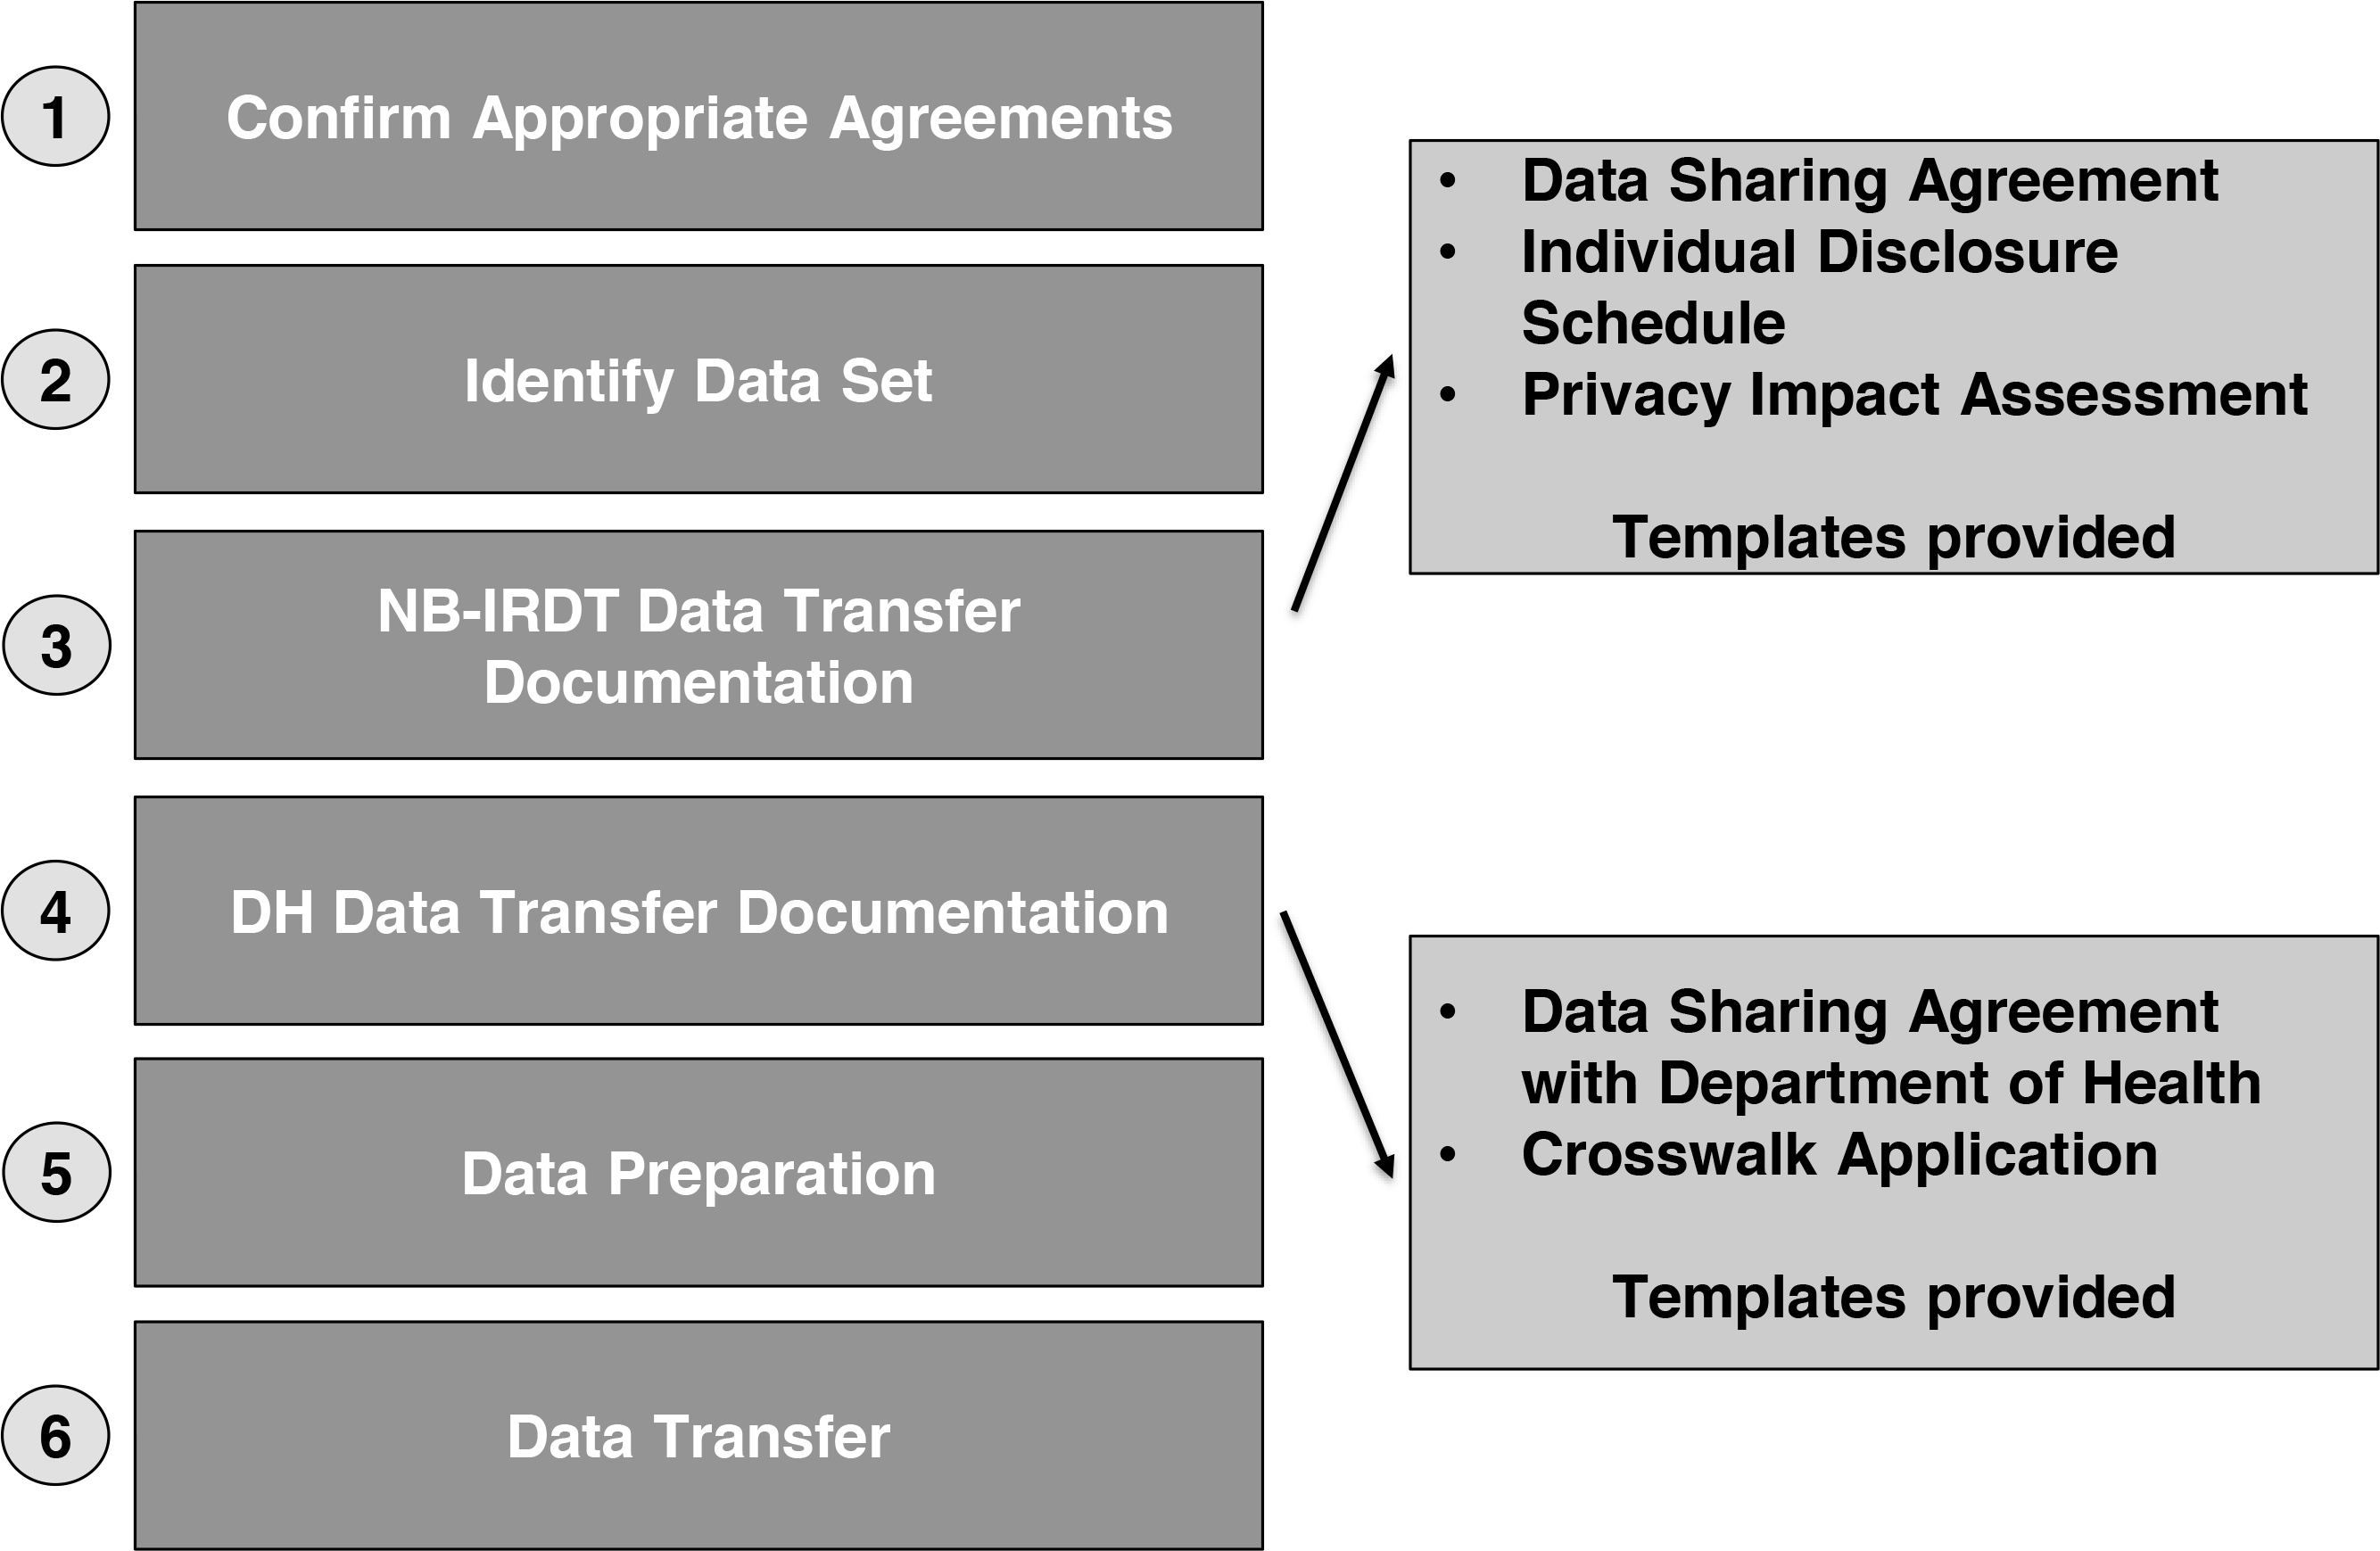
\includegraphics[width=1\linewidth]{./figures/nbirdtfigure1} \caption{Data transfer to NB-IRDT}\label{fig:nbirdtfigure1}
\end{figure}

These principles were made operational through several legal agreements and legislative changes. First, changes were made in 2012 to the PHIPAA\index{PHIPAA} \citep{governmentofnewbrunswick2009}, NB's provincial legislation covering appropriate use of an individual's personal health information, which allowed for the creation of a provincial research data center and defined such an entity as a data custodian. Foundational legal agreements between UNB and the Department of Health (acting as a signatory on behalf of the province) established NB-IRDT as a research data center and defined rights, responsibilities, and reporting requirements, including an originating agreement and an operational agreement both signed in 2013 (the text of which are confidential). The concept of a provincial research data center did not previously exist and so was defined through this legislation as a facility that could provide secure data access to third parties for research purposes. Following that there were other changes to PHIPAA and to the Medical Services Payment Act\index{Medical Services Payment Act}, commonly known as the Medicare Act\index{Medicare Act} \citep{governmentofnewbrunswick2017}, to allow the Medicare number to be used for data matching purposes in 2015. The next major legislative change was entitled An Act Respecting Research\index{An Act Respecting Research} \citep{governmentofnewbrunswick2017a}. that was proclaimed into law in May 2017. The act defined a clear legal authority for prepared personal information to be transferred to NB-IRDT from many provincial government departments and public bodies by simultaneously modifying numerous other pieces of legislation. Just as importantly, the act also defined the authority for the Department of Health to receive identifying personal information from other agencies but only for the purpose of data matching for disclosure to a research data center.\footnote{See section \protect\hyperlink{nbirdt-making}{Making Data Usable for Research} for a detailed description of a crosswalk file development.} Where the Medicare number was not available in the disclosed data, the Department of Health would use probabilistic matching methods. This was followed by a second Act Respecting Research\index{Act Respecting Research} that was proclaimed in June 2019 and addressed some legislative gaps in the first act.\footnote{See section \protect\hyperlink{nbirdt-institutionalsetup}{Institutional Setup} for the legislative authority for NB-IRDT to operate.} It is worth noting that this pathway to current practice was not predetermined but rather evolved incrementally as successive obstacles and problems arose and were resolved. Similarly, at the time that the concept of a research data center was defined, there was no template for what would be required to establish and operate one and this, too, evolved over time. What was consistent throughout the time period was a commitment to achieving the vision of a research data center as a facility to make available for research linkable data from multiple government departments and public bodies.

\hypertarget{nbirdt-legaluse}{%
\subsection{Legal Context for Data Use}\label{nbirdt-legaluse}}

Disclosure of de-identified personal and personal health information for research purposes is authorized in the NB Right to Information and Protection of Privacy Act\index{Right to Information and Protection of Privacy Act} (RTIPPA) and PHIPAA\index{PHIPAA}, respectively. Access for research purposes is subject to a set of specific yet customizable security safeguards including administrative, physical, and technical practices and procedures.\footnote{See section \protect\hyperlink{nbirdt-fivesafes}{Protection of Sensitive and Personal Data: The Five Safes Framework} for detailed description of safeguards.} These safeguards seek to ensure the confidentiality, security, accuracy, and integrity of all data held in custody. In order to comply with these legislative requirements, NB-IRDT has adopted a set of eleven data privacy and security policies to embed privacy best practices through all data access, use, disclosure, and retention processes.\footnote{See NB-IRDT website \href{https://www.nbirdt.ca/data-privacy-and-security}{Data Privacy and Security} for the complete set of policies.} These best practices are drawn from the Canadian Standards Association's ten privacy principles \citep{governmentofcanada2000a, officeoftheprivacycommissionerofcanada2019}, which mirror the Organization for Economic Co-operation and Development (OECD) guidelines. This embedding of legislation and privacy principles into all data policy and procedures is in itself in keeping with the international best practice of Privacy by Design\index{Privacy by Design}, the incorporating of data protection into all processes, services, and levels of an organization, institution, or service provider \citep{hertzman2012}. By adopting and following these policies, NB-IRDT is able to implement a set of criteria to be met for researchers to become approved users prior to accessing the data. Criteria include legislated safeguard requirements such as criminal record checks, signing of confidentiality agreements, and ongoing participation in privacy training. See Figure \ref{fig:nbirdtfigure2} \emph{NB-IRDT approved user criteria} for an outline of requirements.

Data access for research purposes does not only require scrutiny over potential users but over the potential research and the actual data requested for access. A particular strength of PHIPAA\index{PHIPAA} is its Section 43, which speaks to the disclosure of data for research purposes. Similarly, data access by NB-IRDT staff for data curation purposes is also guided by legislation that defines the purposes for which access is granted.

\begin{figure}
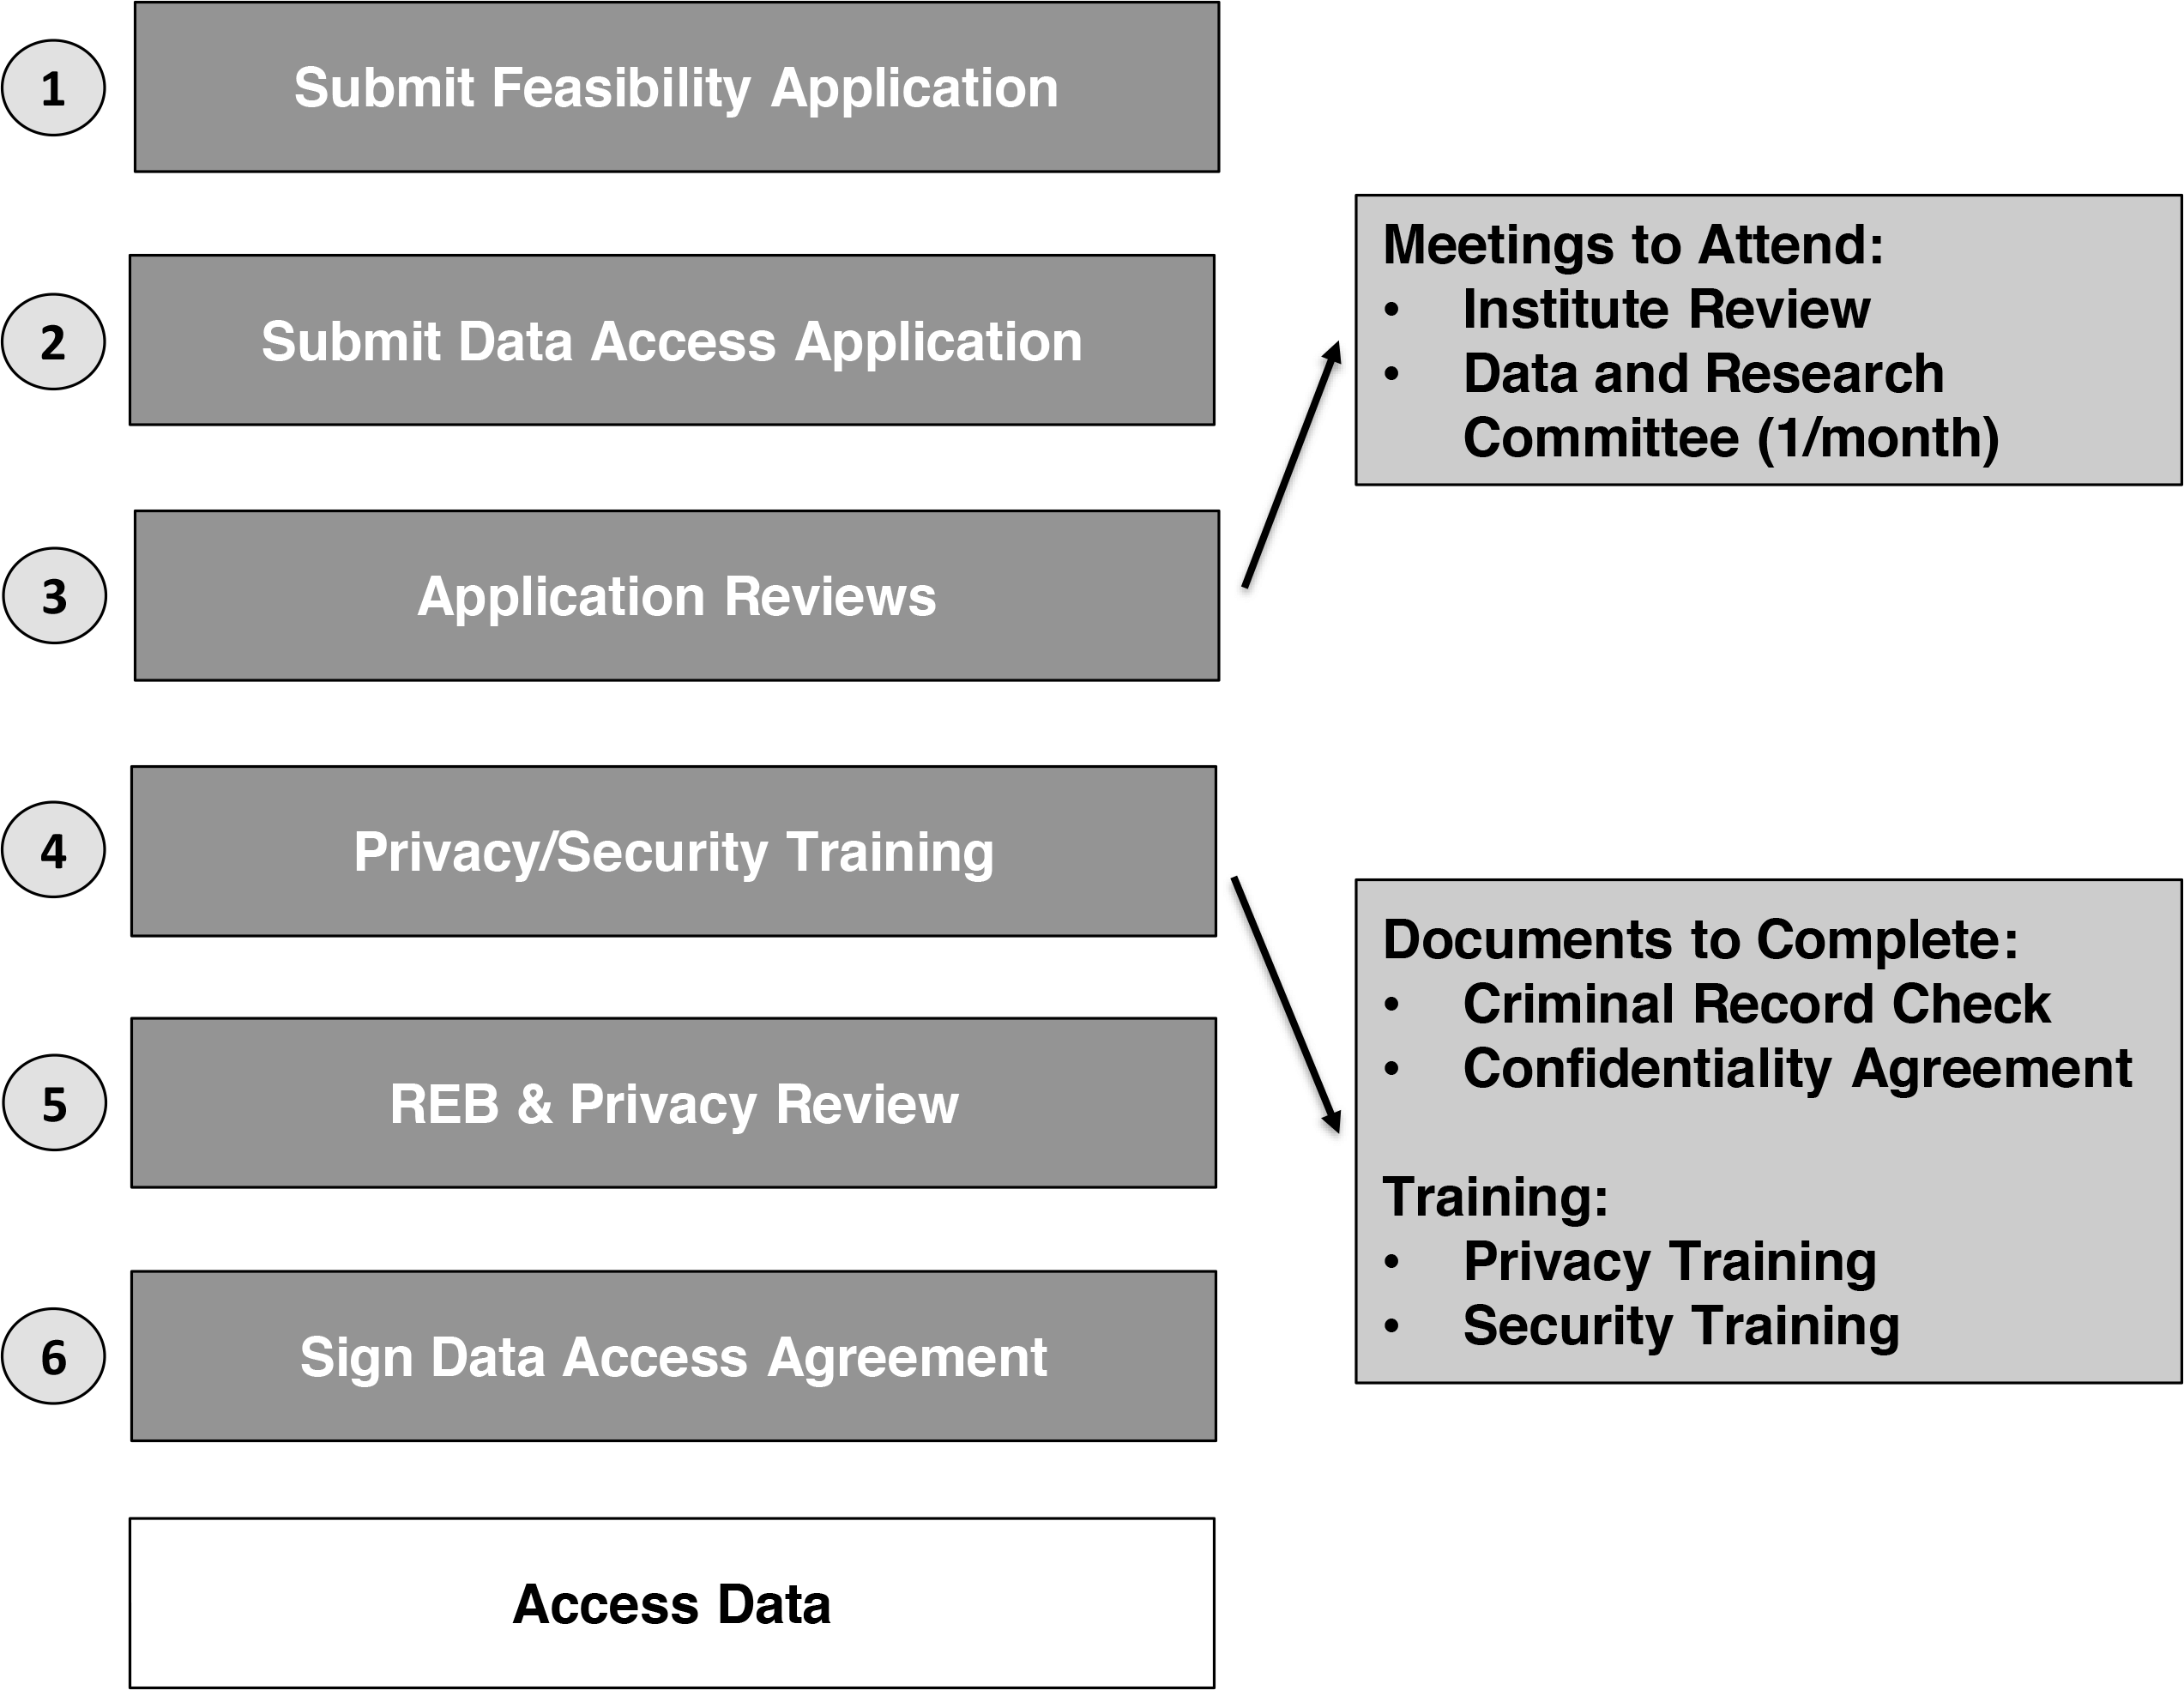
\includegraphics[width=1\linewidth]{./figures/nbirdtfigure2} \caption{NB-IRDT approved user criteria}\label{fig:nbirdtfigure2}
\end{figure}

In recognition of significant contributions that can be derived from research outcomes enabled by research access to administrative data sets, NB legislation includes a consent waiver clause. Custodians may grant access to personal information for research purposes without an individual's consent when it would be unreasonable or impractical for researchers to obtain such consent. While this permission applies to the accessing of de-identified personal information, the impracticality of seeking consent must be justified within the compulsory review process and cannot simply be a matter of inconvenience.

\hypertarget{nbirdt-legalaccess}{%
\section{Legal Framework for Granting Data Access}\label{nbirdt-legalaccess}}

While data sets transferred to NB-IRDT remain under the authority of the disclosing body, the research products that arise from data access are typically the intellectual property of the principal investigator for the project unless otherwise noted in a research contract or agreement. Intellectual property rules must also conform to UNB policy, the basis of which is that research activity undertaken by a faculty member is the property of the faculty member, since NB-IRDT is part of UNB. A standard acknowledgement phrase that must be included in all disseminated research products is required by NB-IRDT. There is no requirement for co-authorship on any research using administrative data on the NB-IRDT platform. In certain circumstances for some data sets provided by a data user (such as data collected by a physician in private practice), the data owner may require co-authorship should another researcher seek to use that user-provided data, but no data received from public bodies carries any such requirement. Furthermore, while most research products remain the intellectual property of the project's principal investigator, there is a general principle that all research undertaken using NB-IRDT data should be made public. Reports undertaken for GNB are posted on the NB-IRDT website following the required embargo period.\footnote{Unless specifically undertaken through a contract, reports for government remain the intellectual property of the researcher. NB-IRDT strongly encourages publication of all research reports but the ultimate decision resides with the author(s). Publication of work undertaken in fulfillment of a contract will depend on the terms of the contract.}

\hypertarget{nbirdt-fivesafes}{%
\section{Protection of Sensitive and Personal Data: The Five Safes Framework}\label{nbirdt-fivesafes}}

\hypertarget{nbirdt-safeproject}{%
\subsection{Safe Projects}\label{nbirdt-safeproject}}

All requests to access administrative data sets held on the NB-IRDT platform begin with submission of a feasibility application. This is an initial review identifying the appropriateness of the requested data sets for the proposed work and the resource requirements to undertake that work. If deemed feasible (sometimes after modification), applicants are invited to submit a complete data access application package to the NB-IRDT project coordinator\index{project coordinator}. Applications are verified for completeness, and NB-IRDT staff are alerted to the pending project.

Following the initial processing, the application undergoes a number of sequential reviews. First, an Institute review is undertaken. This review covers basic privacy compliance, peer to peer review of general methodology with respect to data requirements, appropriateness of data set requests, and confirmation of necessary funding and resource needs.\footnote{In the interests of expediency, the project application process typically begins prior to a contract or MOU being signed, although data analysis does require such an agreement to be in place.} Editing of the application is normally required as a result of this meeting and recommendations are provided in writing to applicants. After concerns and comments are addressed, a meeting of the NB-IRDT Data and Research Committee (DRC) is scheduled. In attendance at the DRC meeting are committee core members, representatives of the original data business owner of requested data sets (optional), the data access applicant, and representative Institute staff. During this meeting original data business owners are given the opportunity to inquire about the appropriateness of requested data access, data usage, and to discuss the proposed project in detail. These are productive discussions often resulting in important modifications to the applications. Applicants receive a written summary of the meeting's outcomes and recommendations. Once necessary edits have been made, the applicant is then invited to apply to the University of New Brunswick Research Ethics Board (UNB REB) for research project approval. The condition of approval by a research review body is just one among many safeguards required for legislative compliance.\footnote{The UNB REB, defined by the Tri-Council\index{Tri-Council}, carries out the role of the research review board. The Tri-Council\index{Tri-Council} is composed of Canada's three federal research agencies: the CIHR\index{CIHR}, the Natural Sciences and Engineering Research Council of Canada\index{Natural Sciences and Engineering Research Council of Canada} (NSERC), and the Social Sciences and Humanities Research Council\index{Social Sciences and Humanities Research Council} (SSHRC). The Tri-Council authors the \emph{Tri-Council Policy Statement: Ethical Conduct for Research Involving Humans (TCPS or the Policy)} \citep{governmentofcanadainteragencyadvisorypanelonresearchethics2020} governing all research involving human subjects inclusive of secondary use of administrative data.}

The REB reviews data access applications for their compliance to six requirements laid out in Article 5.5 of the Policy for secondary use of identifiable information without consent of the original contributors. In addition, the REB also seeks compliance with the UNB University Policy on Research Involving Humans\index{University Policy on Research Involving Humans} (UPRIH) \citep{officeofresearchservicesuniversityofnewbrunswick2011}. Evidence of mitigation to resolve any concerns or risks identified by any previous REB reviews in relation to the proposed project must be submitted with the REB application.

REB requirements include ensuring the following conditions are to be met: do the risks of data access outweigh any potential intrusion of privacy; has it been determined that the research cannot be accomplished without the access; will the data be provided in its most de-identified form; are the appropriate safeguards to protect privacy of individuals and security of the data in place; and will access and dissemination of research results be consistent with the purposes for which the access was granted. See Figure \ref{fig:nbirdtfigure3} \emph{NB-IRDT data access for researchers} for an outline of the process at NB-IRDT.

While in general, projects submitted to UNB REB require at least one research team member to be affiliated with UNB, this is not required for projects submitted to NB-IRDT where only secondary data access is being requested. Following the REB review, the application is then systematically reviewed against legislation for privacy compliance by the NB-IRDT privacy officer\index{privacy officer}. Finally, a letter of support is prepared from the institute director\index{institute director} and the application and supporting documentation are submitted to the University Office of Research Services where it is given approval by the vice president (research).

Following data access approval, principal investigators (PIs) are required to enter into a data access agreement\index{data access agreement} with the University of New Brunswick. This agreement reiterates the appropriate safeguards to be followed, establishes the accountability of the PI for the research team, and confirms commitment that the use and disclosure will be consistent with approved access.

For data sets already at NB-IRDT, the typical processing time from receipt of the feasibility request to signing the data sharing agreement is about three months. Actual processing times can be significantly longer when they involve the incorporation of new data sets from the researcher or a public body. As the volume of applications continues to increase, NB-IRDT is adapting its application process to meet the demand. For example, in February 2020 an expedited review process was introduced by the Data and Research Committee (DRC) to review applications likely to be straightforward. In this process, applications are sent for review to a subset of the DRC and review results communicated to the researcher by e-mail. Currently, NB-IRDT staff are undertaking a broader process improvement evaluation to consider all stages of the application process, to identify potential bottlenecks, and to determine how to address these potential delays.

\begin{figure}
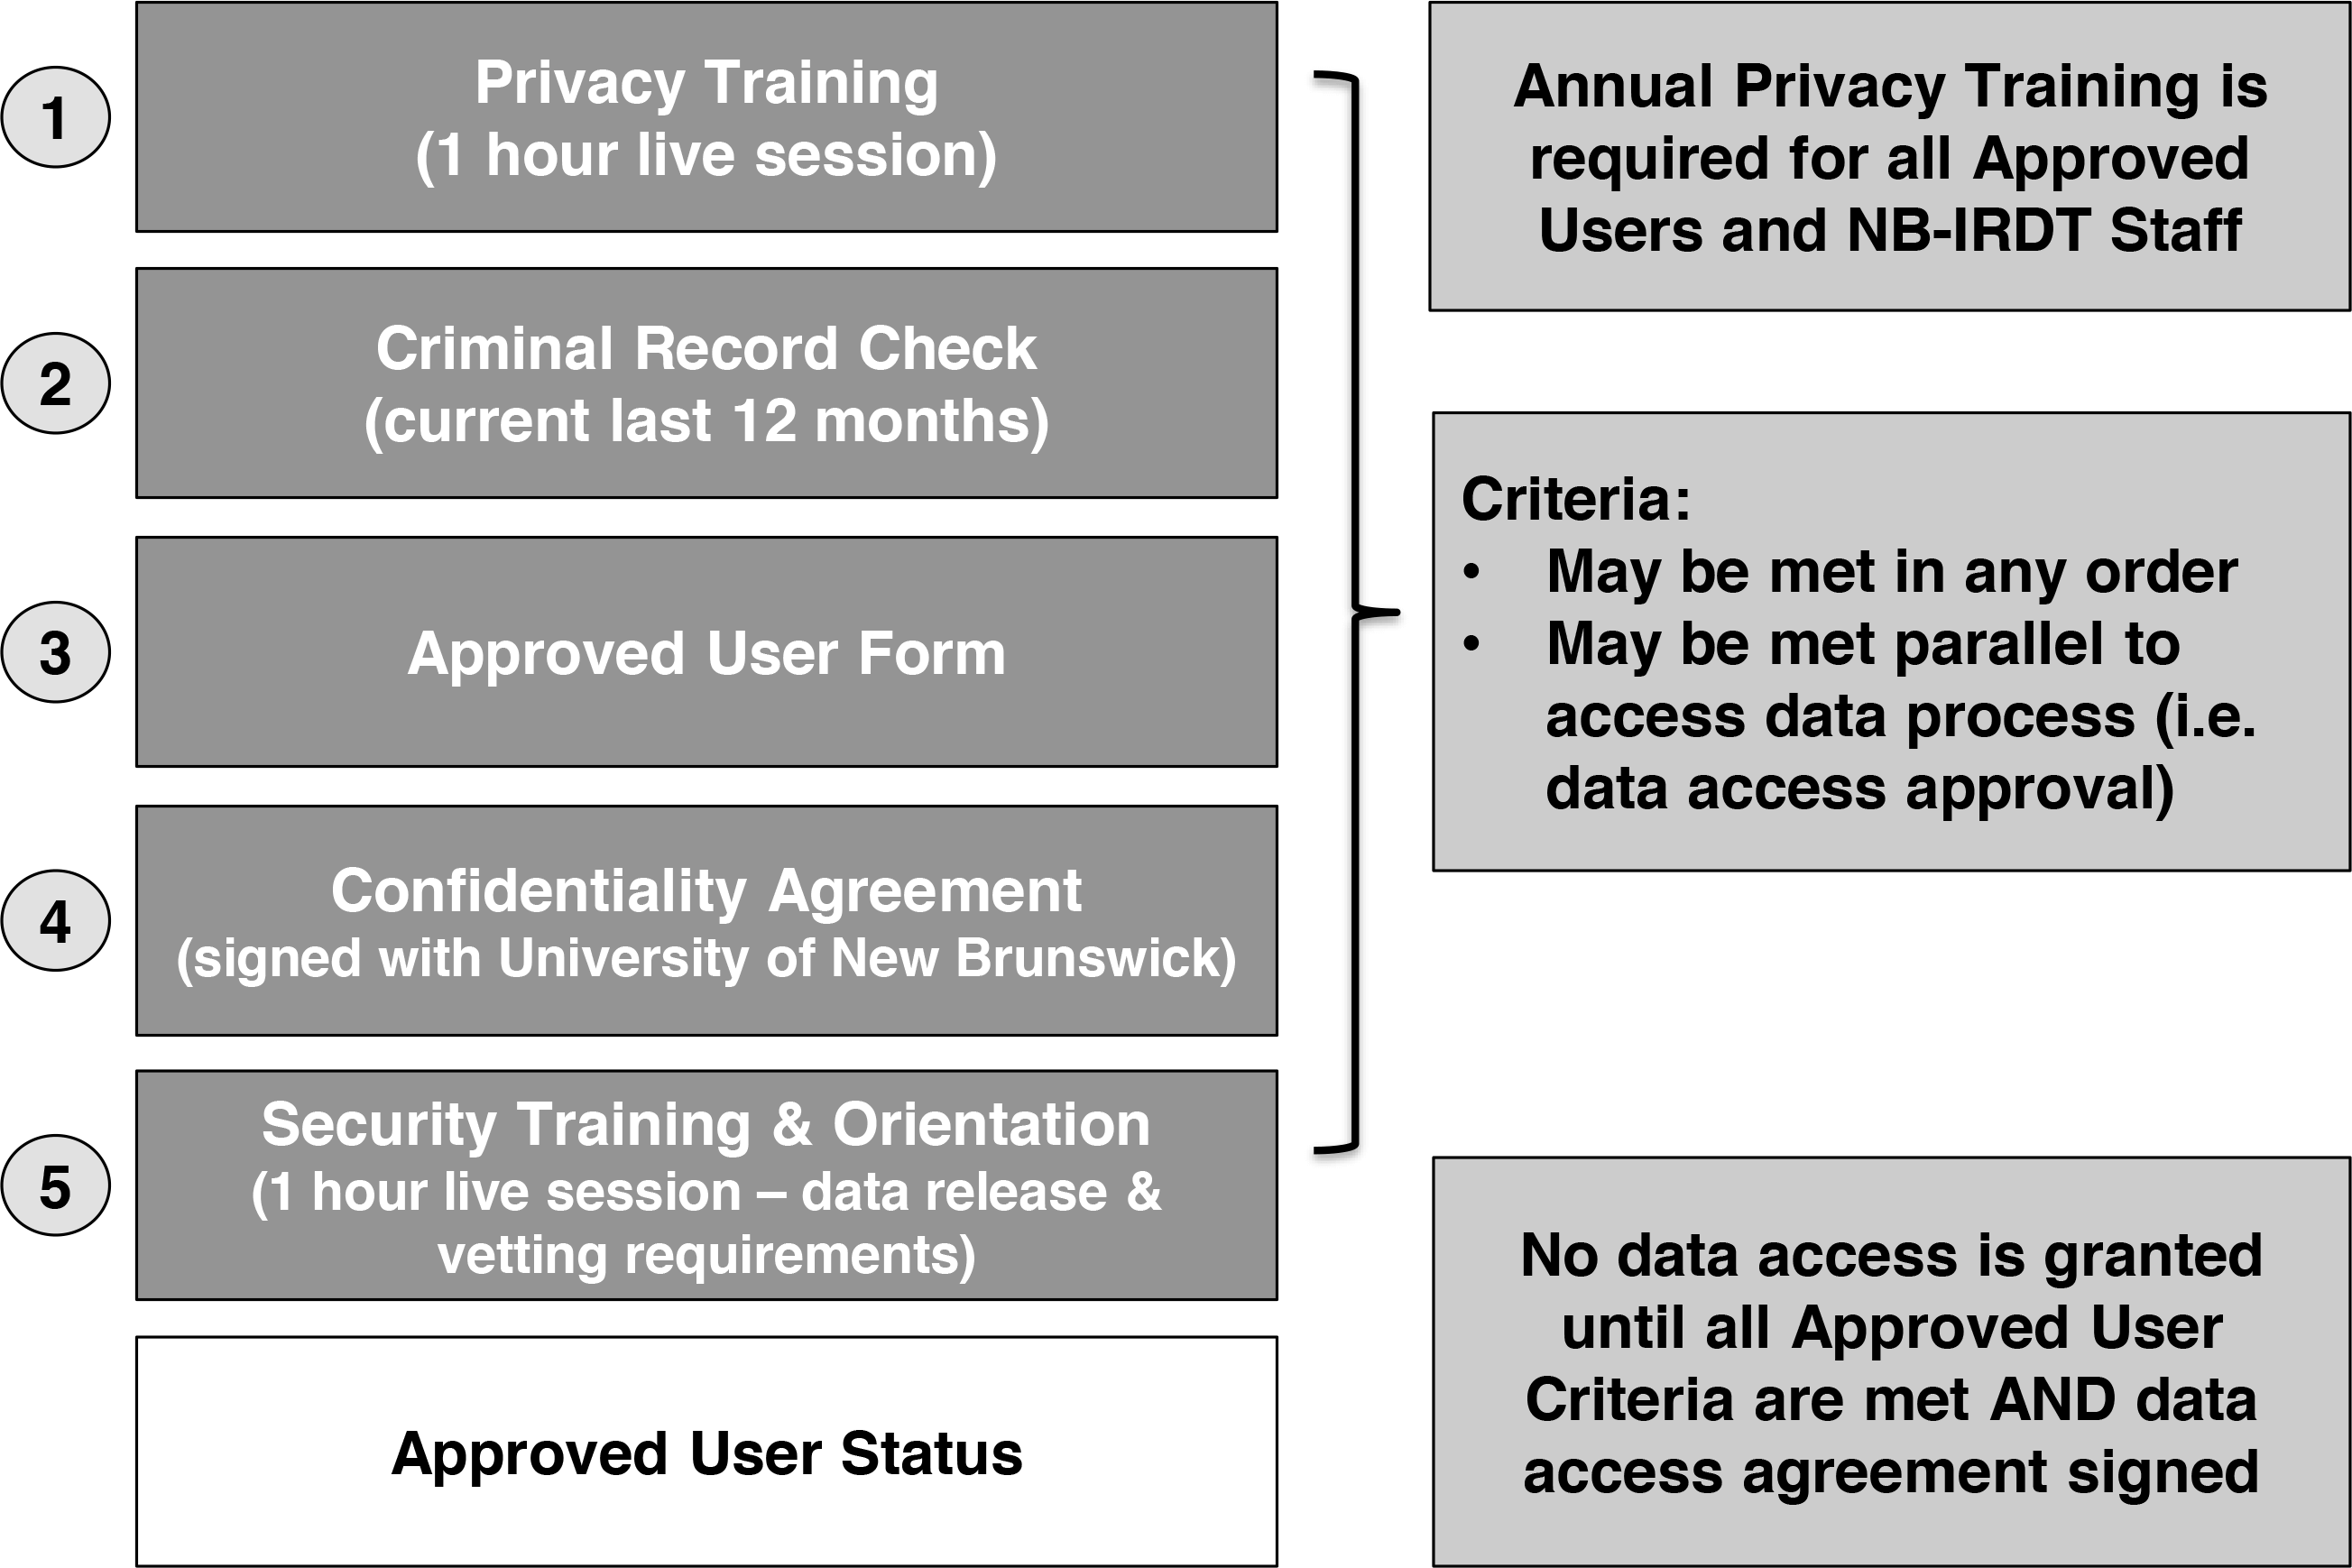
\includegraphics[width=1\linewidth]{./figures/nbirdtfigure3} \caption{NB-IRDT data access for researchers}\label{fig:nbirdtfigure3}
\end{figure}

\hypertarget{nbirdt-safepeople}{%
\subsection{Safe People}\label{nbirdt-safepeople}}

All potential users of the NB-IRDT and staff members regardless of their roles (e.g., managers, support staff, data analyst\index{data analyst}, etc.) are required to follow a set of administrative safeguards in keeping with legislative requirements. These include evidence of a criminal record check completed within twelve months of the data access application and a signed confidentiality agreement indicating their commitment to adhere to NB-IRDT policies, privacy principles, and best practices.\footnote{See section \protect\hyperlink{nbirdt-legaluse}{Legal Context for Data Use} for legal and policy details.} Individual users and staff must also participate in a one-hour administrative data privacy training session and an additional data security and results vetting request session to remind users of their obligations. Training sessions are offered twice monthly through an online platform and content is revised in keeping with legislation and privacy best practices. The principal investigator for each project is also required to provide a current curriculum vitae and sign a data access agreement\index{data access agreement} with the University. This agreement attests to their responsibility for their actions and those of their research team members in relation to data access and use while in an open project relationship with NB-IRDT.\footnote{Though not codified, sufficient criteria may include one or more of the following: successfully completing projects using administrative data, securing competitive research funding, or using administrative data for program evaluation or research as part of regular employment.} Penalties for violating NB-IRDT policies will vary depending on the nature and frequency of the action but can include warnings and temporary or permanent suspension of data access. More severe violations would be the purview of the University of New Brunswick Office of Research Services.\footnote{It is notable that NB has no statistics act that may prescribe criminal sanctions for data breach such as fines or imprisonment. An example of such an act in Canada is the Canadian Statistics Act\index{Statistics Act} of 1985 \citep{governmentofcanada1985}} Additionally, all staff and approved users must attend annual privacy training sessions to review the material covered, as part of the project approval process, as a mitigating measure against potential privacy breach or incidents.

A unique strength of the New Brunswick legislation is its lack of requirement for data access applicants to hold an academic affiliation. In lieu, it is the role of the review processes to determine whether access adheres to permitted research purposes. The lack of a specific academic affiliation requirement applied in tandem with the obligatory safeguards embedded in the NB-IRDT data access application process means that opportunities for research work extend beyond traditional academic boarders. This permits access to users from government, non-profits, and private sectors.

\hypertarget{nbirdt-safesettings}{%
\subsection{Safe Settings}\label{nbirdt-safesettings}}

Currently, users must access their project files on site in one of three secure facilities (a central and two satellite sites) in NB and access is gained through the assignment of both a dedicated entry card and unique PIN. Inside the secure facility, several additional physical and technical safeguards are in place. Approved users and staff may only access data sets within specific project folders. Each user has their own unique username and password, and a separate log-in and password is required for each project such that a user cannot access two project data sets\index{project data set} at the same time. All workstation ports are disabled except for USB ports for a mouse and keyboard that can only accept these devices. Within the central location, workstations operate on a closed network and there is no connection to external networks (i.e., there is no internet or wireless capabilities). Project work or data cannot be saved to the local workstations and can only be saved to the local server. Security software runs in the evening and every weekend to ensure no data or files are saved to local hard drives or desktops. Users in the satellite sites use thin clients and at no time are users working on local workstations. All sites are alarmed and locked with deadbolts after working hours. Project data set access at the two satellite sites is through a zero-client model by which the satellite locations are connected to the central server by dedicated secure fiber-optic cable. Thus, the network is air gapped with respect to the wider internet. The zero-client framework for the satellites was implemented mainly for confidentiality reasons so that NB-IRDT data files remain on the secure servers in Fredericton. Zero-client analysis can also offer significant computational advantages and NB-IRDT is in the process of planning for eventual migration of the Fredericton workstations to the same zero-client environment. Approved users may access the facility during regular business hours of 9:00 a.m. to 5:00 p.m. while staff are permitted limited after-hours access based on job requirement.

Mobile devices are not permitted inside the secure facilities and approved users and staff are asked to take phones calls and similar outside of the facilities. Two exceptions are permitted: emergency IT work conducted by the NB-IRDT systems administrator\index{systems administrator} and immediate assistance to approved users provided by data analysts\index{data analysts}. These exceptions are monitored by staff surveillance and incidents are reported to the NB-IRDT privacy officer\index{privacy officer} for mitigation.

As a final physical safeguard, all textbooks and related print material deemed necessary for project work within the lab as well as physical notes must be vetted through the NB-IRDT senior data analyst\index{senior data analyst}. Approved users and staff must send such documentation to the senior data analyst electronically for vetting and addition to appropriate project folders. Written notes made while in the lab are taken on designated blue paper, may not be removed from the secure facilities, and are securely shredded when no longer needed.

Physical access within the secure facility is governed by staff roles and responsibilities. Approved users are permitted to work using one of the eleven workstations in the main lab of the secure facility. Limited access to a lockable, inner staff-office is available to the NB-IRDT data manager\index{data manager}, systems administrator\index{systems administrator}, and as needed the data analysts\index{data analysts}. The NB-IRDT senior data analyst\index{senior data analyst} is stationed in an adjacent, inner office where the server and media safe are housed. Only the senior data analyst and systems administrators have keys to this room. The server is held in a locked cage and both the server and the safe are bolted to the floor. The safe requires two individuals to be present for opening: one person with a key and one with a passcode. ~~

In the NB-IRDT data lab, researchers have routine access to Stata, R, SAS, ArcGIS, and SPSS and may request other commercial software packages to be installed. Data access fees are based on a standard fee schedule that specifies rates per project and per hour of work, so total project fees vary depending on the scope of work.

\hypertarget{nbirdt-safedata}{%
\subsection{Safe Data}\label{nbirdt-safedata}}

All personal information and personal health information, regardless of format (identifiable or de-identified, i.e., pseudonymous) or stage of the data life cycle, is treated and given an equal level of protection. There are no distinctions or classes of data in the legislation for data that are considered personal information or personal health information. This lack of distinction, with the exception of truly anonymous data (i.e., no possibility of re-identification) that is not covered under the legislation, ensures consistent safeguards are followed and reduces the potential risks of identification, re-identification, inappropriate use, access, or disclosure.\footnote{A curious feature of privacy legislation in NB, which may result in some confusion, is that in the English version of the legislation the term used is `de-identified' but in the French version the term used is `anonymous'. Since NB is an officially bilingual province, all legislation must be in both French and English.}

Project data sets\index{project data set} are prepared files that include only those data elements required to undertake the project and those approved for release to the researcher. The Institute ID\footnote{See section on \protect\hyperlink{nbirdt-making}{Making Data Useable for Research} for more details} is replaced by a study number; these numbers are specific to projects so they cannot be used to link multiple data sets. Since the project data set is a single data set that comprises approved data elements from one or more NB-IRDT data set(s) assembled by the senior data analyst\index{senior data analyst} working as the database administrator\index{database administrator}, the researcher is not required to do any data linkage or merging. In the review stage, the researcher was required to provide a rationale for why each data element would be required for the project. The prepared file will contain only those variables approved for access or derivations from underlying variables whose release would be considered especially sensitive. For example, a full postal code (often sufficient to identify an individual street in urban areas) is rarely required by researchers for their project work. Instead, the prepared data set may have only the first three digits of the postal code but also include derived measures of travel distances. Similarly, derived variables may include duration of stay in hospital but only the month and year of admission to hospital are included.

\hypertarget{nbirdt-safeoutput}{%
\subsection{Safe Outputs}\label{nbirdt-safeoutput}}

Once project work is complete, a researcher must add a vetting request file to their project folder for review by the NB-IRDT senior data analyst\index{senior data analyst}. Output requested for vetting and release may include regression results, cross-tabular results, graphs, and related output. Person-level data cannot be released for any reason. The senior data analyst applies both a basic set of vetting rules (i.e., no release of cell counts less than five) as well as a more exhaustive set of vetting practices and considerations to avoid residual disclosure of identifiable information if other output has been released previously. Vetting rules are based on those used in the Statistics Canada research data centers though the rules are adapted for NB administrative data.\footnote{Vetting rules are not published but are discussed with the research team at project launch as part of the mandatory information sessions for researchers with newly approved projects.} Although multiple disclosure requests are permissible for a particular project, researchers are discouraged from doing so because of resource implications and the fact that earlier releases may restrict what can subsequently be released. For output that does not meet requirements for disclosure, the senior data analyst will typically consult with the research team to discuss options such as reformatting tables, aggregating categories, or the use of random rounding. Only the NB-IRDT has the capacity to download and release project results to the principal investigator. Questions and challenges to the vetting procedure or results approved for release can be raised with the NB-IRDT Vetting Committee whose membership includes the NB-IRDT director\index{director}, privacy officer\index{privacy officer}, a research associate\index{research associate}, and at least two data analysts\index{data analysts}. Decisions are recorded for transparency and future reference. The NB-IRDT \emph{Dissemination of Research Findings Policy} requires all research projects to build in a thirty-day embargo period prior to the release of any first-release research results. During this time, Institute staff and the DRC members who approved the data access application are able to review the material or publication for appropriate data use, access n as well as privacy compliance.

\hypertarget{nbirdt-replicability}{%
\section{Data Life Cycle and Replicability}\label{nbirdt-replicability}}

\hypertarget{nbirdt-accessfile}{%
\subsection{Preservation and Reproducibility of Researcher-Accessible Files}\label{nbirdt-accessfile}}

The data life cycle of all platform and project data sets\index{project data set} files must comply with both legislative requirements for data access for research purposes and the standards set by privacy principles. To ensure compliance, NB-IRDT follows a set policy on data retention, destruction, and restoration. NB-IRDT administers two data life cycles.

First, the data life cycle of all data sets transferred to NB-IRDT are retained and made accessible within the terms and conditions prescribed in their related written agreements. The conditions speak to the limiting of access for research purposes and the requirement for a stated rationale for data access as well as to the terms of ongoing retention for the lifetime of the Institute. The agreements also refer to potential retraction or partial retraction. Terms of retraction are generally in relation to a data business owner's data quality concerns or noncompliance on the institute's part. In good faith and in recognition of the researcher process, however, clauses permitting project data set\index{project data set} access until project closure have been secured in most agreements.

The life cycle of project data sets\index{project data set} are administered following set parameters. Project data sets for approved research projects are created once all criteria for approved users' access have been met and the principal investigator signs a data access agreement\index{data access agreement} with the university. The start date of the project aligns with the approval date from the REB. Generally, research ethics approval is for three to five years with annual progress reports submitted to the REB.

Access to dedicated project folders is for the life of the project or until the end of the project's research ethics approval, whichever comes first. Project extensions are permitted through renewal of REB approval. Access to projects data sets is withheld until REB confirmation is received.

While the REB process governs project data access, complete project data sets\index{project data set} as well as vetted results are stored on the NB-IRDT secure server for a period of three years immediately following the project end date. The three-year timeline is considered sufficient for researchers to make revisions to academic papers or other reports for dissemination as required as part of a peer review process for publication.

Physical receipts are issued to data business owners for all data sets transferred to the secure custody of NB-IRDT. In addition, any necessary returns to business owners (e.g., corrupted files on delivery) are also given a return receipt. Should a data business owner or custodian request disposition of a data set from the NB-IRDT servers (e.g., at the close of an information manager agreement) a certificate of secure destruction is provided. A bonded third-party shredding service who has been vetted for standard compliance completes destruction of physical media. A certificate of secure destruction is provided.

\hypertarget{nbirdt-generatedfile}{%
\subsection{Preservation and Reproducibility of Researcher-Generated Files}\label{nbirdt-generatedfile}}

In addition to the retention of the complete data set and results, project specific syntax, coding, and related information are retained for an additional seven years. Secure disposition of this file takes place following the seven years.

New Brunswick legislation does not permit access to personal information or personal health information for any longer than is needed to complete the purpose for which permission to access was granted. As a result, project data sets\index{project data set} cannot be retained for an unlimited time nor can they be reused for purposes other than originally permitted. This does not preclude, however, the retention of syntax that does not include variables or results information. Approved users seeking to reuse such information may request its release through the secure vetting request process. They may also choose to add such information to the shared code banks\index{code banks} accessible to all approved users for particular data sets.

\hypertarget{nbirdt-sustain}{%
\section{Sustainability and Continued Success}\label{nbirdt-sustain}}

\hypertarget{nbirdt-outreach}{%
\subsection{Outreach}\label{nbirdt-outreach}}

Outreach is vital to the continued operation of NB-IRDT in at least four ways. First, NB-IRDT has regular reporting requirements to original data business owners, custodians, and funders around data access, finances, and related operational issues. Second, NB-IRDT engages with other prospective data custodians (for example, other government agencies) about the benefits of sharing data with NB-IRDT and how the Institute can support them in that process. Third, NB-IRDT engages with prospective research partners across the spectrum including academics, clinicians, trainees/students, and members of both non-profit and private sectors who may be interested in accessing linkable administrative data to support their work. Fourth, NB-IRDT engages in extensive knowledge translation and dissemination activities in order to demonstrate the impact that work undertaken by NB-IRDT's own research staff---academic publications and presentations, reports for government, graduate student theses, and contracted research---is having in supporting evidence-informed policy and practice. \footnote{See NB-IRDT website at \href{https://www.nbirdt.ca/publications}{Research, Publications} and \href{https://www.nbirdt.ca/nbirdt-events}{News, Events} for links to previous public events.}

Outreach activity takes many forms. Disseminating research outcomes to funders uses both formal and informal channels. Formal channels include annual reports, annual research days specifically for particular departments and public bodies, and an annual open house conducted collaboratively with GNB's Executive Council Office. The most recent open house was attended by close to 100 GNB employees. The PETL research day, for example, includes research presentations on those projects indicated to be of most interest to PETL's senior management team and is attended by the deputy, assistant deputy ministers, program directors, and departmental research staff. Informal channels include the production research bulletin reports that are posted on the NB-IRDT website and academic and public presentations.

Research impact is communicated to the public through public showcases and events, through the production of press releases, and through social media, with research results presented in a readily understandable form for the intended audience.

Outreach to prospective partners and users also employs both formal and informal methods. Tailored information sessions have been given to almost every GNB Department, usually at the invitation of the Deputy Minister. Similar sessions have been given to other public bodies, non-profit organizations, and private sector and trade groups provincially, nationally, and internationally. For example, NB-IRDT is a central component of NB's engagement with pharmaceutical companies interested in investing and researching in NB at the annual Biotechnology Innovation Organization (BIO) international trade convention. At the other end of the spectrum, NB-IRDT has conducted several facilitated sessions with non-profit groups and charities on NB-IRDT's capacity to support needs assessments and program impact evaluations. One ongoing collaboration is with Living SJ, a nonprofit organization that supports charities in Saint John, NB. This collaboration, funded by GNB, will see NB-IRDT supporting data collection, transfer, and program analysis for up to twelve SJ-based charities.

For academic users, including students and trainees, information on what is available and how to get access is communicated through online resources and in-person information sessions conducted across the province. Venues include health, social science, and statistics departments of NB's universities, both NB medical schools (for clinicians and medical students), and research groups' centers in the regional health authorities.

\hypertarget{nbirdt-revenue}{%
\subsection{Revenue}\label{nbirdt-revenue}}

The funding model for NB-IRDT's operations has been evolving since its launch in 2015. Initial infrastructure funding came from a Canada Foundation for Innovation\index{Canada Foundation for Innovation} (CFI) grant but funding to establish NB-IRDT as an institute came through the MSSU\index{MSSU} research agreement jointly funded by CIHR\index{CIHR} and the Department of Health. CFI\index{CFI} funding covered renovations to build a secure lab at UNB, hardware and software purchase, installation, and configuration; MSSU funding covered salaries for the first personnel hired to develop the range of policies and procedures that needed to be in place before a research data center could operate. MSSU funding also covered associated expenses including external threat and risk assessments and privacy impact assessments. These direct costs to establish NB-IRDT do not include the significant value of in-kind work provided by a host of GNB personnel to establish NB-IRDT as a data custodian. This work took the form of drafting legislation, co-designing legal agreements, extensively contributing to and reviewing policies and procedures, and establishing (in law and in practice) the process by which the Department of Health would take on the function of data matching for all data destined for transfer to NB-IRDT. This was a major undertaking given the expectation that NB-IRDT would eventually host all research-relevant data on NB residents.

As of 2020, NB-IRDT has revenue from grants, contracts, and fee-for-service work of approximately CA\$2.5 million, which reflects increasingly diversified funding sources. While UNB provides in-kind support for the physical operation of the facility (space, utilities) and for financial, human resources, and legal services, all other operating costs must be met from external sources. An increasingly important source of operating costs is data development. The extraction, curation, and transfer of data from government departments and public bodies is often resource intensive, and those agencies rarely have personnel to devote to the work of data preparation for NB-IRDT. To address this NB-IRDT has seconded data specialists into various agencies to undertake the bulk of this data preparation work.

MSSU\index{MSSU} funding is still a significant proportion of revenue, but it is supplemented with a number of other revenue lines. These include contributions to operating and research costs from other line departments at GNB, funding from other research grants and contracts awarded to the NB-IRDT director\index{director}, researchers and affiliated scientists, and fee-for-service. Prospective users are informed of the requirement for cost recovery upon making contact with NB-IRDT. The fee schedule is an internal document and is not publicly available. Fees for each project are computed based on estimated hours of work plus a facility access fee. Researchers undertaking their own data analysis would pay only for data preparation and project and data access fees. Fee levels reflect the cost per hour of the research services requested including administrative support. Applicable fees may be lower than published levels in certain circumstances at the discretion of the director if the research collaboration offers additional benefits to NB-IRDT (for example, through the addition of new data sets to the NB-IRDT platform or by establishing a new partnership with a public body). It should be noted that work undertaken through MSSU as a provincial priority project or as part of an established funding agreement with a government partner does not typically involve additional fees. All academic and public sector users face the same fee schedule regardless of academic affiliation, although there is a higher fee schedule for users from the private sector to compensate for the use of publicly funded infrastructure.

\hypertarget{nbirdt-metrics}{%
\subsection{Metrics of Success}\label{nbirdt-metrics}}

Since its originating date, the NB-IRDT has been collecting metrics in two main categories: the development of the Institute's data assets and its capacity to support research. While some of the metrics captured are required under the terms and conditions of agreements, others have been invaluable performance indicators identifying service gaps and growth opportunities for NB-IRDT to become a sustainable research data center.

Without administrative data sets secured from government departments, public bodies, and other key data business owners, NB-IRDT would not be able to fulfill its mandate. The Institute's capacity to grow its data platform and make those data available for research and program evaluation requires ongoing attention. Numerous hours and events have been spent networking and fostering relationships with potential partners. These efforts are indicated in the number of data sets received as well as in their depth of coverage and diversity. Both the number of partnerships and data sharing agreements are recorded in addition to the actual number of data sets made available on the platform for data access application. As of early 2020, excluding data sets held under information manager agreements, there are approximately forty data sets currently available for data access application with an additional forty at various stages of transfer and receipt. In addition, several of these are coming from first-time partnerships under master data sharing agreements indicating partner intent to share additional data sets.

A second key area of measurement for NB-IRDT examines its ability to support research. Statistics are captured along the entire data access application process, to inform key stakeholders of capacity and for internal performance measures and process improvement. Measuring starts with the number of feasibility applications submitted followed by the full data access applications that are submitted. In turn, the number of applications actually pursued to full project status is also recorded. By way of example, in 2019, sixteen feasibility requests were reviewed resulting in twelve data access applications leading to six approved data access projects as of the end of the year. Most of the feasibility requests will eventually become approved applications although delays may arise for various reasons. As of June 2020, ten projects are also currently in the beginning of the data access application process. By default, the number of full applications submitted also reflect the number of institute and privacy reviews conducted and the number of Data and Research Committee meetings held. They do not reflect the number of major amendments to projects, which are triggered by changes to the approved data access. These amendments can range from changes in research team membership (which requires REB approval) to changes in project scope or the addition of data sets held by partners not previously consulted; thus, additional REB approval DRC meetings are needed. There were twelve such amendments in 2019, however, the overall need continues to decrease as researchers become more familiar with administrative data research work and the support documentation for data sets strengthens.

Additionally, the length of time between process stages is measured. This measure serves as both an indicator to prospective researchers as well as a performance measure for project coordination and management. Application processing time from start to finish, often the first question asked by potential researchers, has proved to be the most challenging of measurements. Though internal processes are examined and modified for efficiency, the barrier is controlling for external factors. External factors include unforeseen delays in data sets transfer triggered by specific project needs, incompletion of safeguard measures by potential researchers, scheduling of review meetings with numerous partners at the table, researchers' completion of necessary edits or updates following reviews and application resubmission, delays in REB submissions, and working around funding requirements and deadlines. As internal processes continue to improve, ongoing communication and education about these processes to researchers, as well as addressing their responsibility to fulfill application requirements, is key decreasing overall application time.

Audits of data sets accessed and data project activity are a requirement of data sharing with NB-IRDT as well as a legislated safeguard. Reporting at this level allows not only for the monitoring of appropriate data access but also provides partners with an indicator of the usage of their data. A final metric for NB-IRDT is the number of disseminated research results or outputs from data access. Not only are the requests for first-time disclosure captured but also efforts are made to identify subsequent publications or sharing of results in additional formats beyond the relationship with NB-IRDT.

\hypertarget{about-the-authors-3}{%
\section*{About the Authors}\label{about-the-authors-3}}
\addcontentsline{toc}{section}{About the Authors}

\href{https://www.unb.ca/faculty-staff/directory/nbirdt/curtis-maillet-donna.html}{Donna Curtis Maillet} has been the Privacy Officer for the NB Institute for Research, Data and Training since it originated in 2015. In addition to a background in library and information sciences, she holds an interdisciplinary PhD and has research work experience in science and technology studies and legal pluralism. Dr.~Curtis Maillet has been a part-time lecturer in sociology and public policy at St Thomas University since 2014.

\href{https://www.unb.ca/faculty-staff/directory/arts-fr-economics/mcdonald-ted.html}{James Ted McDonald} is a professor of economics at the University of New Brunswick in Fredericton. He holds a PhD in economics from the University of Melbourne, Australia. He is the founding director of the NB Institute for Research, Data and Training, New Brunswick's only provincial administrative data center. He is the chair of the Canadian Research Data Centre Network Academic Council, he is a member of the CRDCN Board, and he is the academic director of the NB Statistics Canada Research Data Centre. Dr.~McDonald is also on the executive committee of Health Data Research Network Canada and is the New Brunswick lead of the Maritime SPOR SUPPORT Unit (MSSU). Dr.~McDonald is a UNB research scholar for 2020 to 22 and previously held that title in 2012 to 14. In 2019 he was co-winner of the Mike McCracken award for Economics Statistics, awarded by the Canadian Economics Association.

\emph{Curtis Maillet and McDonald each contributed equally to all sections of this case study.}

\begin{invisible}
This is a workaround for citations in footnotes, please ignore.
@governmentofcanada1985
\end{invisible}

\putbib

